% Gemini theme
% https://github.com/anishathalye/gemini

\documentclass[final]{beamer}

% ====================
% Packages
% ====================

\usepackage[T1]{fontenc}
\usepackage{lmodern}
\usepackage[size=custom,width=120,height=72,scale=1.0]{beamerposter}
\usetheme{gemini}
\usecolortheme{gemini}
\usepackage{graphicx}
\usepackage{booktabs}
\usepackage{subfigure}
\usepackage{tikz}
\usepackage{amssymb}
\usepackage{amsmath}
\usepackage{pgfplots}

% ====================
% Lengths
% ====================

% If you have N columns, choose \sepwidth and \colwidth such that
% (N+1)*\sepwidth + N*\colwidth = \paperwidth
\newlength{\sepwidth}
\newlength{\colwidth}
\setlength{\sepwidth}{0.025\paperwidth}
\setlength{\colwidth}{0.3\paperwidth}

\newcommand{\separatorcolumn}{\begin{column}{\sepwidth}\end{column}}

% ====================
% Title
% ====================

\title{Panviral Pepseq: A Highly Multiplexed Serological Diagnostic}

\author{Zane Fink\inst{1} \and Jason Ladner\inst{1}}

\institute[shortinst]{\inst{1} The Pathogen and Microbiome Institute at Northern Arizona University}

% ====================
% Body
% ====================

\begin{document}

\begin{frame}[t]
\begin{columns}[t]
\separatorcolumn

\begin{column}{\colwidth}

  \begin{block}{Abstract}

Viruses represent a diverse and ubiquitous challenge to the immune system, and a record of these encounters is preserved within our antibody responses. 
Understanding the diverse antiviral immune response has important implications for both epidemiology and immunology, 
but our capacity for characterizing this response has been historically limited due to the low throughput nature of the available assays. 
To circumvent these limitations, we are developing a high-throughput approach for serological characterization that begins with a custom set of oligonucleotides (oligos),
which are ultimately linked to the peptides they encode, in order to allow for direct interaction with serum antibodies.
To aid in the design of these oligos, we have developed algorithms to optimize coverage of a given set of viral proteins using fewer oligos than current algorithms.
By treating the design of these libraries as an instance of the weighted set cover problem, 
we can iteratively select the oligos that best represent the potential epitopes within a given reference set. 
Using these algorithms, we were able to cover an equal amount of peptide diversity with $20\%$ fewer oligos. 
By increasing the efficiency of design algorithms, we are able to cover more viral diversity within a single assay, 
greatly increasing the sensitivity of a single assay.

\end{block}


\begin{alertblock}{Objectives}
  \begin{itemize}
  \item \textbf{Design} an oligo library for Ab-PepSeq that broadly
    covers viruses that infect humans/mammals.
  \item \textbf{Create} algorithms for the efficient coverage of
    \emph{linear epitopes} (i.e., in as few oligos as possible).
  \item \textbf{Implement} these algorithms in an open source
    easy-to-use software package that is freely available for public use.
  \end{itemize}
\end{alertblock}
  % \begin{block}{Hypothesis}
  %   \begin{itemize}
  %   \item By treating the design of an oligonucleotide library as an instance
  %         of the weighted set cover problem, we can cover a grater range of epitope diversity
  %         in a smaller set of designed oligos.
  %   \end{itemize}

  % \end{block}
  \begin{block}{Background: What is PepSeq?}
    \begin{figure}
      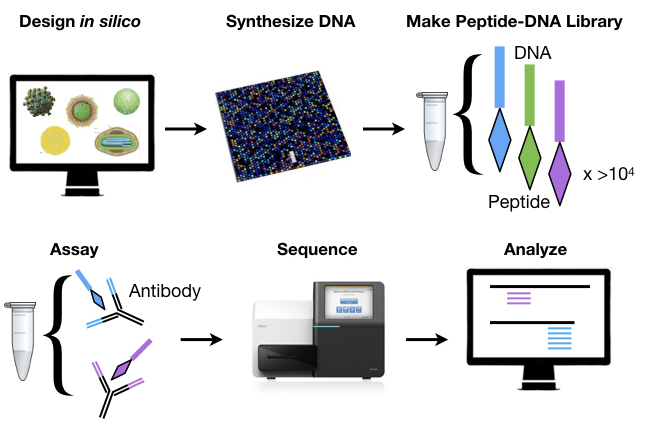
\includegraphics[width=0.6\colwidth]{figures/Overview.jpeg}
      \label{fig:library}
    \end{figure}
    \begin{itemize}
    \item Synthesize $100,000$s of DNA oligos that represent a diverse set of viral proteins.
    \item Serum antibodies used to enrich for recognized peptides
    \item Next-Generation Sequencing used for bulk characterization of enriched peptides.
    \item In this work we focus on the first step: \emph{Design in Silico}.

    \end{itemize}
  \end{block}
\end{column}

\separatorcolumn



\begin{column}{\colwidth}

\begin{block}{The Set Cover Problem}
  Consider a set $\mathcal{U}$ of elements, and a set $S$ of $k$ sets, where
  $\bigcup_{1 \leq i \leq k}S_i = \mathcal{U}$. We seek to cover the elements of $\mathcal{U}$ in as few
  sets of $S$ as possible.
    \begin{figure}
      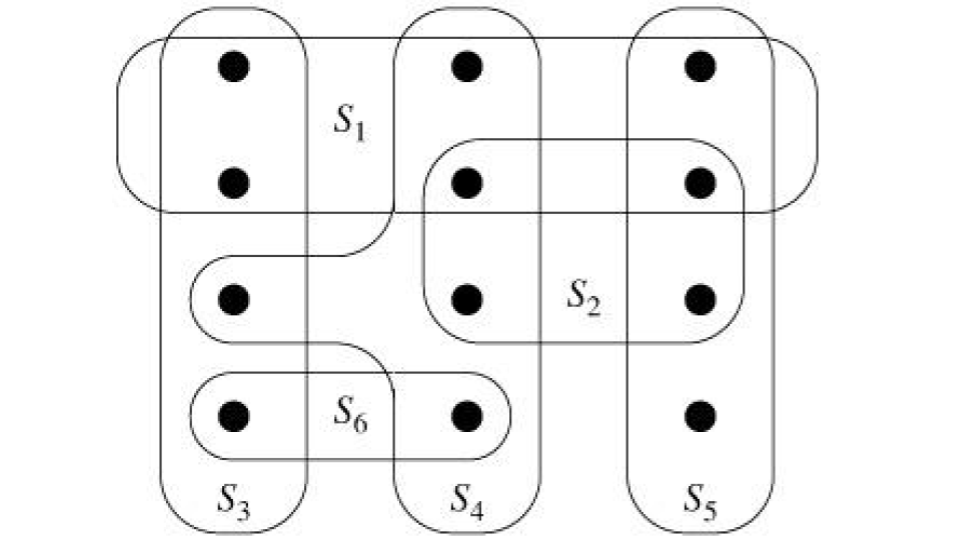
\includegraphics[width=0.5\colwidth]{figures/set_cover.png}
      \label{fig:library}
      \caption{The Set Cover Problem}
    \end{figure}
    \begin{itemize}
      \item How we do cover all of the elements (black dots) of the above in as few sets as possible?
      \item \textbf{Greedy Algorithm}: Choose the largest set of uncovered items, the items in this set are now considered \emph{covered} and are no longer considered.
    \end{itemize}
\end{block}

\begin{block}{The Set Cover Problem As Applied to PepSeq}
    \begin{figure}
      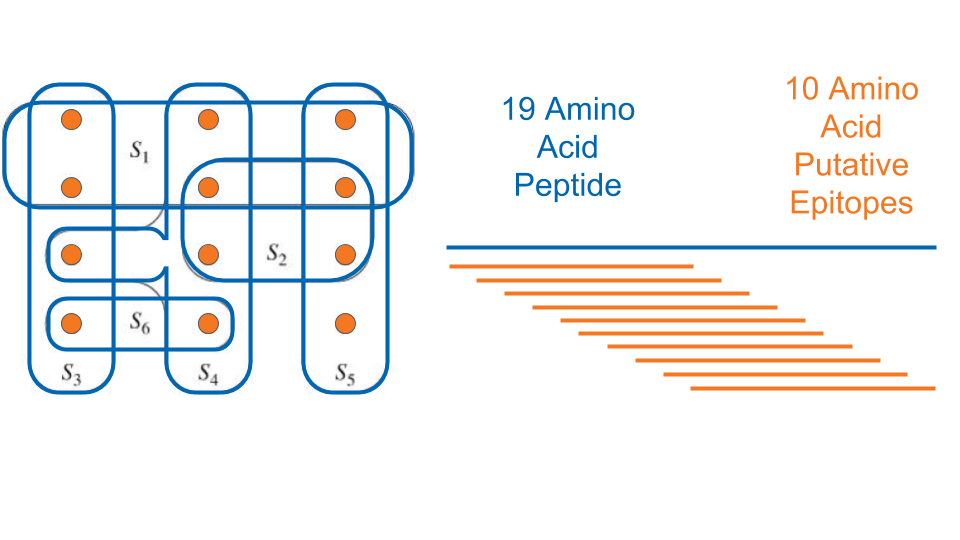
\includegraphics[width=0.7\colwidth]{figures/set_cover_oligo.png}
      \label{fig:library}
      % \caption{}
    \end{figure}
    \begin{itemize}
      \item Here we consider our Universe the set of $10$-mer linear epitopes in a set of viral proteins.
      \item We try to cover these epitopes using as few $19$-mer oligos as possible.
      \item Note that a single $19$-mer can cover up to $10$ unique $10$-mer linear epitopes.
    \end{itemize}


\end{block}
\end{column}

\separatorcolumn


\begin{column}{\colwidth}
  \begin{block}{Large Datasets Need to Be Clustered to Ensure Reasonable Runtime}
    \begin{figure}
      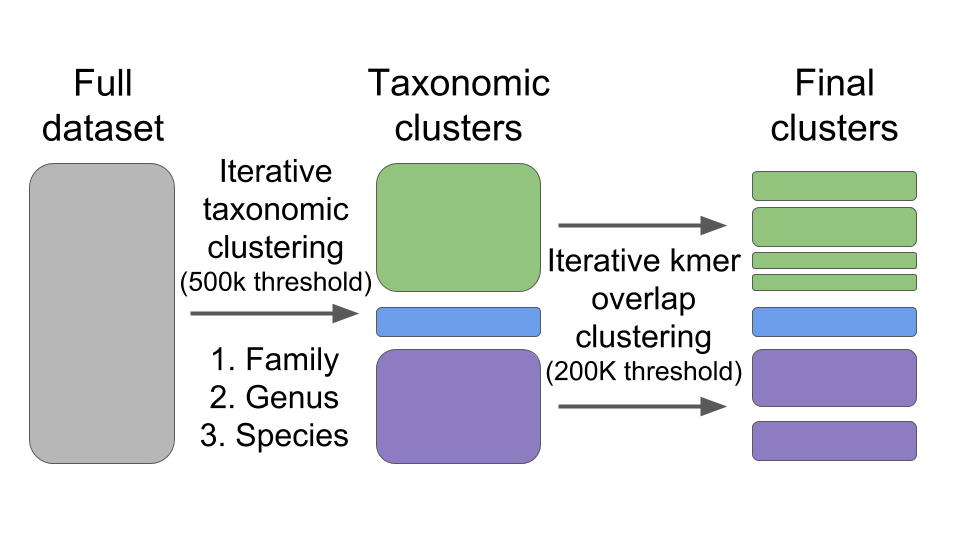
\includegraphics[width=0.5\colwidth]{figures/clustering.png}
      \caption{Visual Depiction of Clustering Process}
      \label{fig:clustering}
    \end{figure}
    \begin{itemize}
    \item Input data of $>1,000,000$ viral proteins is too large to run all at once in a reasonable amount of time,
      so clustering is used to break data down into more manageable pieces.
    \item Two Stages of clustering: \textbf{Taxonomic} and \textbf{Kmer Based}
    \item Taxonomic: Few shared oligos between different taxonomic hierarchies,
      clustering doesn't result in loss of sensitivity
    \item Kmer Based: Clustering by kmers creates clusters of similar sequences,
      good for our approach.
    \end{itemize}

  \end{block}

  \begin{block}{Results}

    \begin{figure}
      \subfigure[Design Algorithm vs. Total Number of Oligos] {%
        \label{fig:total_oligos}
        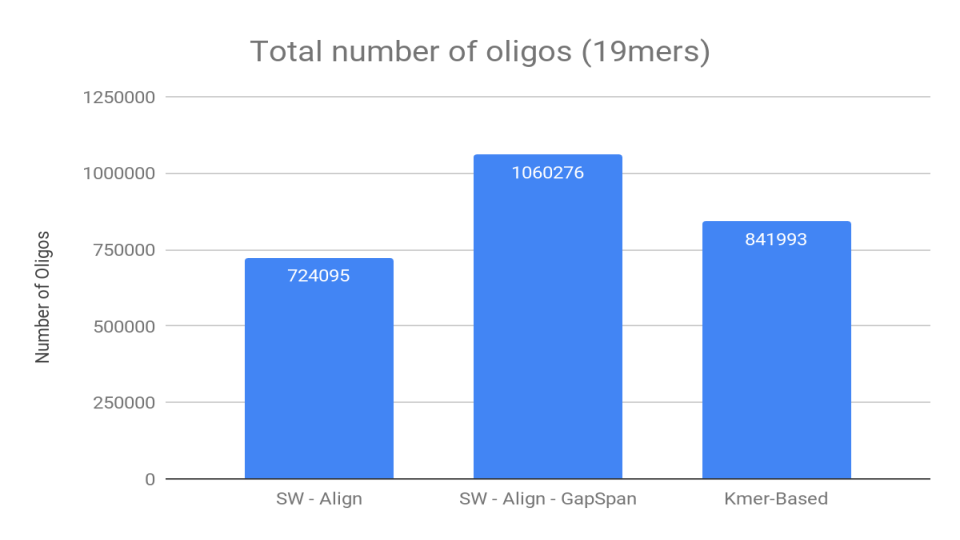
\includegraphics[width=0.55\colwidth]{figures/total_num_oligos.png}
        }
        \qquad
        \subfigure[Design Algorithm vs. Percent Coverage of $10$-mer Epitopes]{
          \label{fig:percent_coverage}
        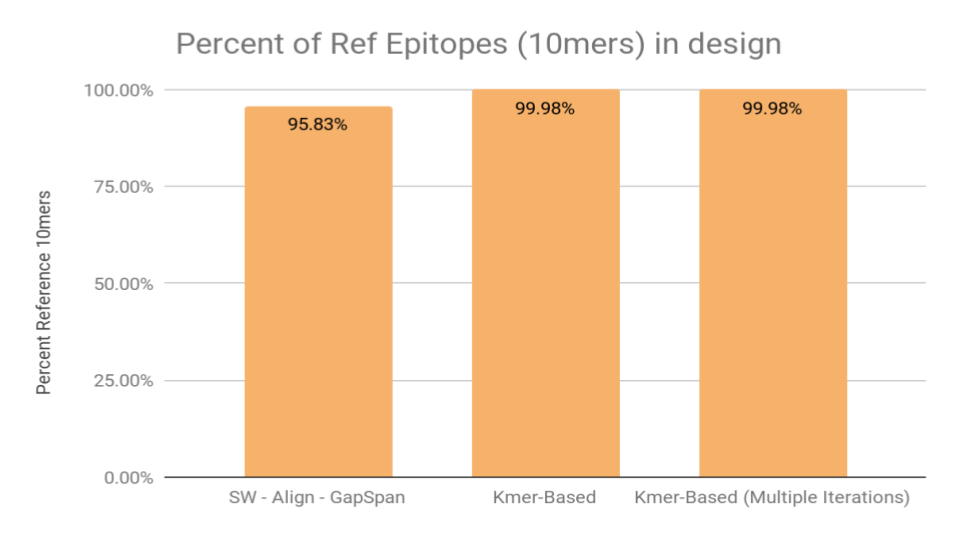
\includegraphics[width=0.55\colwidth]{figures/percent_ref_epis.png}
        }
    \end{figure}

  \end{block}


\end{column}

\separatorcolumn
\end{columns}
\end{frame}

\end{document}
